\chapter{Lecture 7}

This lecture is about \texttt{Unsupervised Clustering
[Hierarchical clustering, K-means, GMM, Gapstatistics]} where chapter \texttt{ESL Chapter 14.3} should be looked upon.

\begin{itemize}
  \item Similarity and dissimilarity measures
  \item K-means clustering
  \item Hierarchical clustering
  \item Gaussian mixture
  \item Validation and model selection
\end{itemize}

\section{Cluster analysis}

Separating or clustering observations, and the intuitive but vague definition:

Given an underlying set of points, partition them into a collection
of clusters so that points in the same cluster are close together,
while points in different clusters are far apart.

The purpose for this is seeing structure in data, and gaining an understanding. We could also have a dimensionality reduction or outlier detection.



\subsection{Proximity Matrices}

In what sense are points close in one cluster and far from points in
another cluster?

Similarity takes a large value when points are close.

Dissimilarity takes a large value when points are far apart. This
reflects the distance between observations.

Any monotone-decreasing function can convert similarities to
dissimilarities.

Both similarity and dissimilarity measures can be subjective. For
example comparing the taste of three ice creams.



\subsection{Dissimilarities Based on Attributes}

The Euclidean distance

\[
    d(x_i, x_j) = \sqrt{\sum_{k=1}^{p} (x_{ik} - x_{jk})^2}
\]

is useful for \textbf{quantitative variables}. Note that ordinal variables can be transformed to a quantitative scale. \cite[p.~11]{lecture7}

Then we have the Manhatten distance

\[
    d(x_i, x_j) = \sum_{k=1}^{p} |x_{ik} - x_{jk}|
\]

\textbf{Quantitative variables} and note Manhattan distance also called city block distance.

There is also the Mahalanobi distance

\[
    d(x_i, x_j) = \sqrt{(x_i - x_j)^T \Sigma^{-1}(x_i - x_j)}
\]

The distance is based on data itself and the two points are assumed
to be of the same distribution with equal dispersion $\Sigma$. \textbf{Quantitative variables}

and we also have the Tanimoto distance

\[
    d(x_i, x_j) = \frac{x_i^Tx_j}{x_i^T x_i + x_j^tx_j - x_i^T x_j}
\]

Let the sample x have $x_k = 1$ if it possesses the i'th attribute, and
$x_k = 0$ otherwise.

The ratio of the number of shared attributes to the number possessed
by $x_i$ and $x_j$.

Often used in information retrieval and biological taxonomy - works
well for \textbf{categorical variables.}

lastly we have weighted distances

\[
    d(x_i, x_j) = \sum_{k=1}^{p} w_k d(x_{ik}, x_{jk}), \quad \sum_{k=1}^{p} w_k =1
\]

Give different weight to the p attributes (variables).

Note that setting $w_k = 1/p$ does not necessarily give equal influence
to the attributes.

We would have to normalize with the average distance for the k'th
attribute.

From \cite[p.~504]{friedman2016elements}, we learn that the \textbf{quantitative variables} are defined as:\\

Measurements of this type of variable or attribute
are represented by continuous real-valued numbers. It is natural to
define the “error” between them as a monotone-increasing function
of their absolute difference

\[
    d(x_i, x_j) = l(|x_i - x_j|)
\]

While \textbf{Ordinal variables} are defined as:\\

The values of this type of variable are often represented
as contiguous integers, and the realizable values are considered to be
an ordered set. Examples are academic grades (A, B, C, D, F), degree
of preference (can’t stand, dislike, OK, like, terrific). Rank data are a special kind of ordinal data. Error measures for ordinal variables are
generally defined by replacing their M original values with

\[
    \frac{i - 1/2}{M}, \quad i = 1,..., M
\]

in the prescribed order of their original values. They are then treated
as quantitative variables on this scale.

and \textbf{Categorical variables} are defined as:\\

With unordered categorical (also called nominal) variables, the degree-of-difference between pairs of values must be
delineated explicitly. If the variable assumes $M$ distinct values, these can be arranged in a symmetric $M \times M$ matrix with elements $L_{rr'} = L_{r'r}, L_{rr} = 0, L_{rr'} \geq 0$. The most common choice is $L_{rr'} = 1$ for all $r \neq r'$, while unequal losses can be used to emphasize some errors more than others.

\subsection{Object Dissimilarity}

If the goal is to discover natural groupings in the data, some attributes
may exhibit more of a grouping tendency than others. Variables that are
more relevant in separating the groups should be assigned a higher influence in defining object dissimilarity. Giving all attributes equal influence
in this case will tend to obscure the groups to the point where a clustering
algorithm cannot uncover them.

Often observations have missing values in one or more of the
attributes. The most common method of incorporating missing values in
dissimilarity calculations


\[
    d(x_i, x_j) = \sum_{k=1}^{p} w_k d(x_{ik}, x_{jk}), \quad \sum_{k=1}^{p} w_k =1
\]

is to omit each observation pair $x_{ik}, x_{jk}$ between observations $x_i$ and $x_j$. This method can fail in the circumstance
when both observations have no measured values in common. In this case
both observations could be deleted from the analysis. Alternatively, the
missing values could be imputed using the mean or median of each attribute
over the nonmissing data. For categorical variables, one could consider the
value “missing” as just another categorical value, if it were reasonable to
consider two objects as being similar if they both have missing values on
the same variables

\subsection{Clustering Algorithms}

So unsupervised clustering is that we have data but no information about class belonging. Group data in clusters, and observations that are "near" each other should belong to the same class/cluster. This can help us unveil an unknown structure in data, it is like classification but without an answer.

\subsection{Combinatorial Algorithms}

\subsection{K-means}

We decide how many cluster there should be, this is our "$K$".

The algorithm alternates between two steps, until assignments do not change. We assign each point to the closest cluster center and compute new cluster centers according to the assignments.

From lecture \cite[p.~20]{lecture7} and from \cite[509]{friedman2016elements}, that K-means is intended for situations in which all variables are of the quantitative type and the squared Euclidean distance is chosen as the dissimilarity measure.

K-mean minimizes within-cluster point scatter. One approach is to directly specify a mathematical loss function and
attempt to minimize it through some combinatorial optimization algorithm.
Since the goal is to assign close points to the same cluster, a natural loss function would be

\[
    W(C) = \frac{1}{2} \sum_{k=1}^{K} \sum_{C(i)=k} \sum_{{C(j)=k}} ||x_i-x_j||^2 = \sum_{k=1}^{K} N_k \sum_{C(i) = k} ||x_i-\tilde{x}_k||^2
\]

where $\tilde{x}_k$ is the mean vector of the k'th cluster and $N_k$ is the number of observations in k'th cluster\\

Thus, the criterion is minimized by
assigning the N observations to the K clusters in such a way that within
each cluster the average dissimilarity of the observations from the cluster
mean, as defined by the points in that cluster, is minimized.

\begin{itemize}
  \item For at given cluster assignment C of data points, compute the cluster means $\tilde{x_k}$
      \[
        \tilde{x_k} = \frac{\sum_{i:C(i) = k} x_i}{N_k}, k=1,...,K
      \]
  \item For a current set of cluster means, assign each observation as
      \[
        C(i) = \arg \min\limits_{1 \leq k \leq K} ||x_i - \tilde{x}_k||^2, i=1,...,N
      \]
  \item Iterate above two steps until convergence
\end{itemize}

K is a user input; alternatively BIC (Bayesian information
criterion) or MDL (minimum description length) can be used
to estimate K. Outliers can considerable trouble to K-means

\subsection{Gaussian Mixtures as Soft K-means Clustering}

The E-step of the EM algorithm assigns “responsibilities” for each data
point based in its relative density under each mixture component, while
the M-step recomputes the component density parameters based on the
current responsibilities

\subsection{Example: Human Tumor Microarray Data}

\subsection{Vector Quantization}

\subsection{K-medoids}

In \cite[515]{friedman2016elements} and \cite[p.~20]{lecture7} we have about K-medoids

As you know, k-medoid is based on centroids (or medoids) calculating by minimizing the absolute distance between the points and the selected centroid, rather than minimizing the square distance. As a result, it's more robust to noise and outliers than k-means.

\subsection{Practical Issues}

\subsection{Hierarchical Clustering}

In \cite[520]{friedman2016elements} and \cite[p.~22]{lecture7} we have about Hierarchical Clustering.

\begin{itemize}
  \item Generates a tree of observations
  \item Each level of the tree reflects one number of clusters
  \item From all data in one cluster down to one observation in each cluster.
\end{itemize}

Furthermore

\begin{itemize}
  \item Do not require input of number of clusters
  \item Uses dissimilarity between clusters
  \item Two approaches
  \begin{itemize}
    \item Bottom-up: Agglomerative (commonly used)
    \item Top-down: Divisive
  \end{itemize}
  \item $n - 1$ levels in the hierarchy
  \item At each level perform split or merge which gives largest between group dissimilarity
\end{itemize}

From \cite[523]{friedman2016elements} we let G and H represent two group, where the dissimilarity $d(G, H)$ between $G$ and $H$ is computed from the set of pairwise observations dissimilarities.

There is the \textit{Single linkage} (SL) takes the intergroup dissimilarity to be that of the closest (least dissimilar) pair

\[
    d_{SL}(G, H) = \min_{\substack{i \in G \\ j \in H}} d_{ij}
\]

Single Linkage tends to give unequal cluster sizes.

This is also often called the nearest-neighbor technique. Complete linkage
(CL) agglomerative clustering (furthest-neighbor technique) takes the in-
tergroup dissimilarity to be that of the furthest (most dissimilar) pair

\[
    d_{CL}(G, H) = \max_{\substack{i \in G \\ j \in H}} d_{ij}
\]

Complete Linkage tends to give balanced trees independent of data

From lecture \cite[p.~29]{lecture7} we have the ward-linkage hierarchical clustering

Cluster-cluster distance measured as the increment in within-cluster sum of squares

\[
    d_{\text{Ward}} = \sqrt{n_G n_H \frac{||\bar{x}_G - \bar{x}_H||^2_2}{n_G + n_H}}
\]

where $n_G$ and $n_H$ are the respective number of observations in each group.

Tends to give a good compromise
between balanced/unbalanced
clusters

\textbf{Note:} Hierarchical clustering will always generate a dendrogram, even when data is completely random, so be careful with the interpretation.

\section{The problem of validation}

How the we select the number of clusters.

So the Gap-Statistic, compares the log criterion value with $K$ clusters to the expected log criterion value for uniformly distribute data

\[
    G(K) = \log(U_k) - \log(W_k)
\]

where $U_k$ within cluster dissimilarity, simulated data - mean over 20 samples and $W_k$ within cluster dissimilarity, actual data

Then choose

\[
    K* = \arg \min\limits_k \{K | G(K) \geq G(K + 1) - s'_{k+1}\}
\]

where

\[
    s'_{k+1} = std(\log(U_k)) \sqrt{1 + 1/20}
\]

To obtain an ideal clustering, you should select k such that you maximize the gap statistic. Here's the exemple given by Tibshirani et al. (2001) in their paper, the plot formed by artificial data with 2 clusters. As you can see, 2 is clearly the ideal k, because the gap statistic is maximized at k=2

\begin{figure}
  \centering
  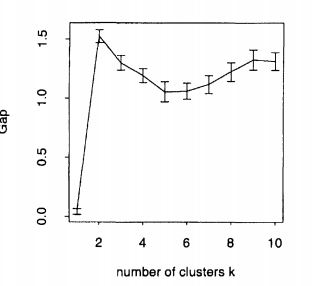
\includegraphics[width=0.9\textwidth]{gapstatK}
\end{figure}

However, in many real-world datasets, the clusters are not as well-defined, and we want to be able to balance maximizing the gap statistic with parsimony of the model.

Assuming that that plot is just going to continue to increase, of course, the results are less useful. So Tibshirani suggests the 1-standard-error method

Which informally is identifying the point at which the rate of increase of the gap statistic begins to "slow down"

\section{Gaussian Mixture Modeling and EM}

Observation from three Gaussian distributions are $X_i \in N(\mu_1, \Sigma_1)$ if $Z_i = 1$, $X_i \in N(\mu_2, \Sigma_2)$ if $Z_i = 2$ and $X_i \in N(\mu_3, \Sigma_3)$ if $Z_i = 3$ and un-observed variables $Z_i$ indicate cluster/distribution, that is $P(Z_i=1) = \tau_1$, $P(Z_i=2) = \tau_2$ and $P(Z_i=3) = \tau_3$ where $\tau_1 + \tau_2 + \tau_3 = 1$

So the parameters in the Gaussian mixture model are

\[
    \Theta = (\tau_1, \tau_2, \tau_3, \mu_1, \mu_2, \mu_3, \Sigma_1, \Sigma_2, \Sigma_3)
\]

and $\bm{Z} = (Z_1, ..., Z_n)$. Then the likelihood is

\[
    \ell (\theta; \bm{x}, \bm{Z}) = \prod_{i=1}^{n} \sum_{j=1}^{3} \mathbb{I}_{\{Z_i = j\}} \tau_j f(x_i; \mu_j, \Sigma_j)
\]

with ML estimate

\[
    \theta_{ML} = \arg \max\limits_{\theta, \bm{Z}} \log \ell (\theta; \bm{x}, \bm{Z})
\]

Finding a solution to $(\theta, \bm{Z})$ is much simplified by the EM-algorithm

The algorithm is a two-step iteration

\textbf{Expectation step:} Define the expectation value

\[
    Q(\theta | \theta^k) = E_{Z | x, \theta^k} L(\theta; x, Z)
\]

\textbf{Maximization step:} Find parameter estimate

\[
    \theta^{k+1} = \arg \max\limits_{\theta} Q(\theta | \theta^k)
\]

First step defines the expectation value of the log likelihood given
observed data, $x$, and current value of the parameter estimate $\theta^k$

Second step chooses optimal $\theta$ given the expectation value
whereupon the procedure is repeated until convergence.

So the GMM EM algorithm has 3 steps

\begin{itemize}
  \item Initialize means $\mu$, covariances $\Sigma$ and mixing coefficients $\tau$
  \item Expectation step: Calculate conditional probabilities $T_{ij}$ for $Z_i$ belonging to cluster $j$ using Bayes formula
  \item Maximization step: Calculate weighted (using $T_{ij}$) mean and covariance estimates $\mu$ $\Sigma$. Calculate mixing coefficient $\tau$ based on mean of weights
  \item Iterate until convergence
\end{itemize}
